%!TEX root = ../main.tex
%%%%%%%%%%%%%%%%%%%%%%%%%%%%%%%%%%
% Links:
%
% Difficulty:
% Companies: 
%%%%%%%%%%%%%%%%%%%%%%%%%%%%%%%%%%


%\begin{figure}
%	\centering
%	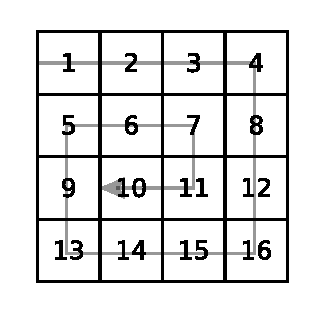
\includegraphics[width=\textwidth]{sources/spiral_matrix/images/example1}
%	\caption[Sample short cpation]{Sample Caption}.
%	\label{fig:spiral_matrix:example1}
%\end{figure}

\section{Spiral Matrix}
\label{ch:spiral_matrix}

\section{Problem statement}
Given a matrix $M$ of size $m\times n$ return a list containing the elements of $M$ in spiral order.
\begin{exercise}
\label{example:spiral_matrix:exercice1}

	%example1
	\begin{example}
		\label{example:spiral_matrix:example1}
		\hfill \\
		Given the matrix shown in Figure \ref{fig:spiral_matrix:example1}  the function returns \inline{1,2,3,4,5,6,7,8,9};
	
		
	\end{example}

	%example2
	\begin{example}
		\label{example:spiral_matrix:example2}
		\hfill \\
		Given the matrix shown in Figure \ref{fig:spiral_matrix:example2}  the function returns \inline{1,2,3,4,8,12,16,15,14,13,9,5,6,7,11,10};
	\end{example}

\end{exercise}
\begin{figure}[t]
    \centering
    \begin{subfigure}[]{0.45\textwidth}
        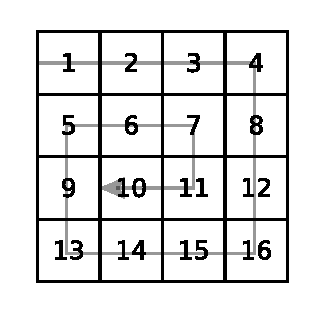
\includegraphics[width=\textwidth]{sources/spiral_matrix/images/example1}
        \caption[]{}
        \label{fig:spiral_matrix:example1}
     \end{subfigure}
    \hfill
    \begin{subfigure}[]{0.45\textwidth}
        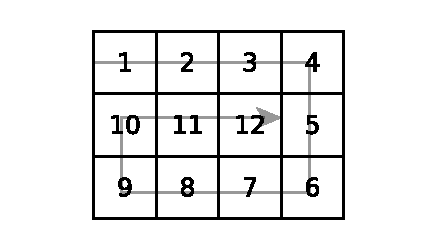
\includegraphics[width=\textwidth]{sources/spiral_matrix/images/example2}
        \caption[]{}
        \label{fig:spiral_matrix:example2}
    \end{subfigure}
\end{figure}



\section{Discussion}
\label{spiral_matrix:sec:discussion}


\subsection{Brute-force}
\label{spiral_matrix:sec:bruteforce}

	\lstinputlisting[language=c++, caption={Sample Caption},label=list:spiral_matrix]{sources/spiral_matrix/spiral_matrix_solution1.cpp}

